\documentclass[conference]{IEEEtran}
\usepackage{cite}
\usepackage{amsmath,amssymb,amsfonts}
\usepackage{algorithmic}
\usepackage{graphicx}
\usepackage{textcomp}
\usepackage{xcolor}
\usepackage{booktabs}
\usepackage{tikz}
\usetikzlibrary{shapes,arrows,positioning,fit,backgrounds}
\usepackage{multirow}
\usepackage{hyperref}
\usepackage{tabularx}
\usepackage{float}

\def\BibTeX{{\rm B\kern-.05em{\sc i\kern-.025em b}\kern-.08em
    T\kern-.1667em\lower.7ex\hbox{E}\kern-.125emX}}

\makeatletter
\newcommand{\linebreakand}{%
  \end{@IEEEauthorhalign}
  \hfill\mbox{}\par
  \mbox{}\hfill\begin{@IEEEauthorhalign}
}
\makeatother

\begin{document}

\title{NeuroCare: Multimodal Early Prediction of Alzheimer's Disease Using Fused Cognitive, EEG, and Acoustic Biomarkers\\
}

\author{
\IEEEauthorblockN{\textbf{Dr. Tejashwini N}}
\IEEEauthorblockA{{Computer Science \& Engineering} \\
{Sai Vidya Institute of Technology}\\
Bengaluru, India \\
tejashwini.n@saividya.ac.in}
\and
\IEEEauthorblockN{\textbf{Suhan SP}}
\IEEEauthorblockA{{Computer Science \& Engineering} \\
{Sai Vidya Institute of Technology}\\
Bengaluru, India \\
suhansp.23cs@saividya.ac.in}
\linebreakand
\IEEEauthorblockN{\textbf{Chirag Shetty A}}
\IEEEauthorblockA{\small {Computer Science \& Engineering} \\
{Sai Vidya Institute of Technology}\\
Bengaluru, India \\
chiragshettya.23cs@saividya.ac.in}
\and
\IEEEauthorblockN{\textbf{Upasana Bharadwaj}}
\IEEEauthorblockA{\small {Computer Science \& Engineering} \\
{Sai Vidya Institute of Technology}\\
Bengaluru, India \\
upasanabharadwaj.23cs@saividya.ac.in}
\and
\IEEEauthorblockN{\textbf{Syeda Manaar Umar}}
\IEEEauthorblockA{\small {Computer Science \& Engineering} \\
{Sai Vidya Institute of Technology}\\
Bengaluru, India \\
syedamanaarumar.23cs@saividya.ac.in}
}

\maketitle

\begin{abstract}
Early detection of Alzheimer's Disease (AD) is critical for timely therapeutic interventions and slowing cognitive decay. However, existing diagnostic paradigms rely heavily on expensive, invasive neuroimaging (PET/MRI) or spinal taps, while single-modality automated screening methods suffer from limited diagnostic robustness across diverse clinical presentations. This paper presents NeuroCare, a non-invasive, multimodal diagnostic decision-support system that synthesizes three distinct biomedical channels: neuropsychological cognitive metrics, 19-channel continuous electroencephalogram (EEG) signals, and acoustic speech biomarkers, enhanced by a computer-vision EEG report digitization engine. Cognitive features are processed from the OASIS longitudinal dataset ($N = 373$), yielding a baseline Regularized Logistic Regression model with 94.64\% validation accuracy (ROC-AUC: 0.9677). 19-channel continuous EEG signals ($N = 88$ human subjects, 1,320 clinical epochs) undergo Butterworth bandpass filtering (0.5--45 Hz), Welch Power Spectral Density (PSD) decomposition ($\delta, \theta, \alpha, \beta, \gamma$), Hjorth complexity analysis, and spectral slowing ratio ($\theta/\alpha$) computation, achieving 77.50\% accuracy (ROC-AUC: 0.8203) using an optimized XGBoost classifier. For clinics lacking digital signal files, a vision skeletonization digitizer parses scanned paper/PDF EEG reports with 95.0\% extraction confidence. Acoustic speech features (80+ parameters including 20 MFCCs, pitch $F_0$, micro-tremor Jitter/Shimmer, and pause ratios) derived from 591 clinical recordings achieve 93.02\% accuracy (ROC-AUC: 0.9806) with a Random Forest model. A constrained Sequential Least Squares Programming (SLSQP) ensemble layer fuses cross-modality probability distributions ($W_{\text{cognitive}} = 0.34, W_{\text{eeg}} = 0.33, W_{\text{speech}} = 0.33$), complemented by SHapley Additive exPlanations (SHAP) for patient-level clinical interpretability. Experimental validation demonstrates that the multimodal ensemble achieves 96.85\% accuracy and an ROC-AUC of 0.9882, surpassing individual single-modality baselines and establishing a scalable, web-deployable framework for non-invasive early AD screening.
\end{abstract}

\begin{IEEEkeywords}
Alzheimer's Disease, Multimodal Fusion, EEG Signal Processing, Acoustic Biomarkers, Cognitive Risk Scoring, Machine Learning, SHAP Explainability, Welch PSD, Hjorth Parameters.
\end{IEEEkeywords}

\section{Introduction}
\IEEEPARstart{A}{lzheimer's} Disease (AD) is a progressive, irreversible neurodegenerative disorder characterized by continuous synaptic loss, neuronal cell death, memory impairment, speech disfluency, and altered cortical electrical activity. As reported by the World Health Organization \cite{who2023}, the global prevalence of dementia is projected to triple by 2050, posing severe socio-economic challenges to global healthcare systems. Pathological hallmarks of AD, such as extracellular amyloid-$\beta$ plaque deposition and intracellular neurofibrillary tau tangles, begin decades prior to overt clinical symptoms. Consequently, identifying patients during the preclinical stage or Mild Cognitive Impairment (MCI) \cite{jack2018}, \cite{sperling2011} represents the crucial window for initiating non-pharmacological interventions, lifestyle modifications, and novel disease-modifying therapies designed to attenuate cognitive decline.

Traditional gold-standard clinical diagnostic workflows rely on Fluorodeoxyglucose Positron Emission Tomography (FDG-PET), volumetric structural Magnetic Resonance Imaging (MRI), and cerebrospinal fluid (CSF) lumbar punctures measuring $A\beta_{42}$ and phosphorylated tau ratios. While highly accurate, these diagnostic procedures suffer from severe limitations: they are physically invasive, cost-prohibitive, associated with radiation exposure or surgical risks, and geographically restricted to specialized tertiary medical institutions. Conversely, first-line screening in primary care heavily relies on standardized paper-based neuropsychological scoring batteries, such as the Mini-Mental State Examination (MMSE) \cite{folstein1975}. Although accessible, standalone cognitive tests exhibit high subjective scoring variability, educational and cultural bias, and practice effects that limit early diagnostic sensitivity.

To democratize early detection, recent computational health research has explored computer-aided diagnosis using single-modality machine learning predictors. Researchers have applied deep convolutional networks to structural brain MRI, computed spectral power distributions from resting-state EEG signals, or extracted acoustic parameters from clinical voice recordings. However, standalone single-modality predictive models exhibit inherent structural vulnerabilities:
\begin{enumerate}
    \item \textbf{Cognitive Profiling Inadequacy}: Static psychological scores capture functional behavioral impairment but fail to detect early pathophysiological electrophysiological or structural neural alterations preceding manifest symptoms \cite{battineni2021}.
    \item \textbf{Bio-Signal Susceptibility}: Continuous EEG recordings are highly sensitive to ocular blink artifacts, electromyographic (EMG) muscle noise, and environmental electrical interference, leading to false-positive classification errors when evaluated in isolation \cite{cassani2018}.
    \item \textbf{Acoustic Biomarker Variability}: Vocal prosody and micro-tremor biomarkers vary significantly across age groups, regional dialects, emotional states, and comorbid respiratory conditions, limiting standalone generalization \cite{cummins2020}.
\end{enumerate}

To address these single-modality vulnerabilities, this paper introduces \textbf{NeuroCare}, an end-to-end, non-invasive multimodal predictive platform. NeuroCare synthesizes three complementary clinical channels: neuropsychological cognitive metrics, 19-channel continuous EEG signal dynamics, and speech acoustic biomarkers. To ensure practical deployability in resource-limited clinics where raw digital signal files are unavailable, NeuroCare incorporates a vision-based paper report digitization engine that automatically ingests scanned hospital EEG reports using optical character recognition (OCR) and morphological skeletonization. The cross-modality probability distributions are integrated using a constrained Sequential Least Squares Programming (SLSQP) soft-voting ensemble, complemented by SHapley Additive exPlanations (SHAP) for transparent, patient-specific clinical decision support.

The primary contributions of this work are summarized as follows:
\begin{itemize}
    \item \textbf{Unified Multimodal Architecture}: Development of a decoupled, multi-tier decision-support system integrating cognitive, neurophysiological (19-channel EEG), and vocal acoustic channels.
    \item \textbf{Computer-Vision EEG Digitization Engine}: Implementation of an automated document rendering, OCR text extraction, and 1-pixel morphological skeletonization pipeline that converts scanned paper/PDF EEG reports into 19-channel continuous microvolt signals with 95.0\% extraction confidence.
    \item \textbf{Optimal SLSQP Ensemble Fusion}: Formulation of a constrained optimization model that dynamically balances cross-modality prediction probabilities ($W_{\text{cog}} = 0.34, W_{\text{eeg}} = 0.33, W_{\text{speech}} = 0.33$), achieving a benchmark validation accuracy of 96.85\% and an ROC-AUC of 0.9882.
    \item \textbf{Patient-Level Explainability}: Integration of SHAP additive feature attribution to provide transparent, interpretable biomarker breakdowns for clinical practitioners.
\end{itemize}

\section{Literature Survey}
Automated diagnostic systems for Alzheimer's Disease have evolved significantly across cognitive scoring, signal processing, vocal biomarker modeling, optical document digitization, and machine learning fusion techniques.

\subsection{Cognitive \& Neuropsychological Assessment}
Early computational diagnostic approaches centered on longitudinal patient tracking and functional assessment scales. Morris \textit{et al.} established the Clinical Dementia Rating (CDR) framework \cite{morris1993}, establishing standardized clinical stages for healthy control ($CDR=0$), mild impairment ($CDR=0.5$), moderate impairment ($CDR=1.0$), and severe dementia ($CDR=2.0$). Marcus \textit{et al.} curated the Open Access Series of Imaging Studies (OASIS) longitudinal dataset \cite{marcus2007}, providing public access to demographic, cognitive (MMSE, CDR), and volumetric brain parameters (nWBV, eTIV, ASF). Tadepalli \textit{et al.} evaluated decision tree and support vector machine (SVM) classifiers on OASIS data, achieving high accuracy in distinguishing advanced dementia \cite{tadepalli2021}. However, as highlighted by Battineni \textit{et al.} \cite{battineni2021}, static cognitive batteries are subject to ceiling and floor effects, making them insufficient as standalone predictors during early preclinical stages.

\subsection{EEG Signal Processing \& Spectral Complexity}
Resting-state electroencephalography (EEG) provides non-invasive, high temporal resolution monitoring of cortical bio-electric activity. Jeong \textit{et al.} demonstrated that AD pathophysiology is characterized by a fundamental shift in spectral power distribution known as ``spectral slowing''---a significant reduction in high-frequency alpha ($\alpha$) and beta ($\beta$) power accompanied by a marked increase in low-frequency delta ($\delta$) and theta ($\theta$) power \cite{jeong2004}. Babiloni \textit{et al.} confirmed that alpha band desynchronization in parietal and occipital electrodes serves as a distinct neurophysiological marker distinguishing AD from Frontotemporal Dementia (FTD) \cite{babiloni2014}. 

Subsequent quantitative EEG studies established that spectral slowing ratios, specifically the theta-to-alpha power ratio ($R_{\theta/\alpha} = P_\theta / P_\alpha$), correlate strongly with cognitive decline severity \cite{blackburn2018}, \cite{horvath2018}. To capture non-linear signal dynamics, Gu \textit{et al.} combined Welch Power Spectral Density (PSD) estimation with Hjorth time-domain parameters (Activity, Mobility, and Complexity) \cite{gu2021}. Utilizing recent public benchmark datasets such as OpenNeuro (ds004504) \cite{miltiadous2023}, researchers have deployed gradient boosting classifiers (XGBoost) and 1D Convolutional Neural Networks (1D-CNNs) on multi-channel EEG epochs to capture subtle cortical disorganization \cite{cassani2018}.

\subsection{Acoustic Voice Biomarkers \& Speech Degradation}
Vocal degradation and linguistic disfluency represent sensitive behavioral indicators of early neurodegeneration. Cummins \textit{et al.} conducted extensive acoustic feature analysis, demonstrating that AD patients exhibit alterations in Mel-Frequency Cepstral Coefficients (MFCCs), fundamental frequency ($F_0$) variations, pitch instability (Jitter), amplitude perturbation (Shimmer), and increased vocal pause durations during standardized picture description tasks \cite{cummins2020}. Fraser \textit{et al.} validated that narrative speech pauses and syntactic complexity reduction correlate with early memory loss \cite{fraser2016}. 

Grisales \textit{et al.} analyzed acoustic micro-tremors and vocal tract impulse responses, demonstrating that high-frequency acoustic perturbations differentiate mild dementia from normal cognitive aging \cite{grisales2021}. Modern speech processing pipelines utilize delta and delta-delta MFCC parameters \cite{lopez2018} along with spectral contrast profiles \cite{pulido2020}. Automated acoustic analyzers employing Random Forest and SVM ensembles have demonstrated superior sensitivity in non-invasive patient screening \cite{konig2015}.

\subsection{Vision-Based Document Extraction \& OCR}
In rural and primary healthcare facilities, digital signal recording hardware is frequently unavailable, leaving clinicians dependent on physical paper chart printouts. Optical Character Recognition (OCR) systems, such as Tesseract \cite{smith2018} and EasyOCR, have enabled automated text parsing from scanned clinical records. Concurrently, computer vision edge detection, adaptive thresholding, and morphological skeletonization algorithms \cite{bradski2008} allow researchers to trace plotted 1D waveform curves from chart images, bridging the gap between legacy paper reports and digital bio-signal processing pipelines.

\subsection{Multimodal Fusion \& Explainable AI (SHAP)}
To overcome single-modality limitations, information fusion frameworks synthesize multi-domain clinical inputs. Achmad \textit{et al.} demonstrated that combining acoustic speech parameters with cognitive test metrics yields higher classification stability than single-modality baselines \cite{achmad2023}. Decision-level fusion schemes, particularly constrained soft voting via Sequential Least Squares Programming (SLSQP) \cite{chen2022}, prevent dominant modalities from overwhelming weak yet complementary bio-signals. Furthermore, clinical adoption of AI decision-support tools requires model transparency. Frameworks utilizing SHapley Additive exPlanations (SHAP), rooted in cooperative game theory \cite{lundberg2017}, allow clinicians to visualize feature attribution scores, ensuring safe and interpretable clinical decision-making \cite{liu2023}.

\section{Methodology}
The proposed \textbf{NeuroCare} system architecture comprises six interconnected functional modules: (1) Cognitive Data Processing, (2) 19-Channel Continuous EEG Signal Analysis, (3) Computer Vision EEG Report Digitization, (4) Acoustic Speech Feature Extraction, (5) SLSQP Multimodal Decision Ensemble Fusion, and (6) SHAP Clinical Interpretability.

\begin{figure}[h!]
\centering
\begin{tikzpicture}[
    node distance=0.85cm and 0.4cm,
    font=\sffamily\scriptsize,
    inbox/.style={draw=blue!80!black, fill=blue!5, rounded corners=3pt, thick, text width=2.1cm, align=center, minimum height=0.75cm},
    layerbox/.style={draw=emerald!80!black, fill=emerald!5, rounded corners=4pt, thick, text width=7.8cm, align=center, minimum height=0.8cm},
    modelbox/.style={draw=indigo!80!black, fill=indigo!5, rounded corners=3pt, thick, text width=2.1cm, align=center, minimum height=0.75cm},
    ensbox/.style={draw=purple!80!black, fill=purple!5, rounded corners=4pt, thick, text width=7.8cm, align=center, minimum height=0.8cm},
    outbox/.style={draw=rose!80!black, fill=red!5, rounded corners=4pt, thick, text width=7.8cm, align=center, minimum height=0.8cm},
    arrow/.style={->, >=stealth, thick, color=gray!80!black}
]

    % Row 1: Inputs
    \node[inbox] (cog_in) {Cognitive Data\\(OASIS Dataset)};
    \node[inbox, right=0.35cm of cog_in] (eeg_in) {19-Ch EEG Signal\\(OpenNeuro / PDF)};
    \node[inbox, right=0.35cm of eeg_in] (sp_in) {Speech Audio\\(WAV Files)};

    % Row 2: Preprocessing Layer
    \node[layerbox, below=0.6cm of eeg_in] (prep_layer) {
        \textbf{Feature Extraction \& Processing Layer}\\
        Cognitive Scaling \;|\; 0.5--45Hz Bandpass, PSD, Hjorth, Vision Digitizer \;|\; MFCC, Pitch, Jitter, Shimmer
    };

    % Row 3: Machine Learning Models
    \node[modelbox, below=0.6cm of prep_layer.south west, anchor=north west, xshift=0.15cm] (m_cog) {Logistic Reg.\\$P_{\text{cognitive}}$};
    \node[modelbox, below=0.6cm of prep_layer] (m_eeg) {XGBoost\\$P_{\text{eeg}}$};
    \node[modelbox, below=0.6cm of prep_layer.south east, anchor=north east, xshift=-0.15cm] (m_sp) {Random Forest\\$P_{\text{speech}}$};

    % Row 4: SLSQP Ensemble Layer
    \node[ensbox, below=0.6cm of m_eeg] (ens_layer) {
        \textbf{Dynamic SLSQP Soft Voting Ensemble}\\
        $P_{\text{ensemble}} = 0.34 P_{\text{cognitive}} + 0.33 P_{\text{eeg}} + 0.33 P_{\text{speech}}$
    };

    % Row 5: Risk Stratification
    \node[outbox, below=0.55cm of ens_layer] (out_layer) {
        \textbf{Risk Stratification \& Clinical SHAP XAI}\\
        Low ($< 35\%$) \;|\; Moderate ($35\text{--}65\%$) \;|\; High ($> 65\%$) Risk
    };

    % Connectors
    \draw[arrow] (cog_in) -- (cog_in |- prep_layer.north);
    \draw[arrow] (eeg_in) -- (prep_layer.north);
    \draw[arrow] (sp_in) -- (sp_in |- prep_layer.north);

    \draw[arrow] (prep_layer.south -| m_cog) -- (m_cog);
    \draw[arrow] (prep_layer.south) -- (m_eeg);
    \draw[arrow] (prep_layer.south -| m_sp) -- (m_sp);

    \draw[arrow] (m_cog) -- (m_cog |- ens_layer.north);
    \draw[arrow] (m_eeg) -- (ens_layer.north);
    \draw[arrow] (m_sp) -- (m_sp |- ens_layer.north);

    \draw[arrow] (ens_layer) -- (out_layer);

\end{tikzpicture}
\caption{System Architecture and Multimodal Processing Pipeline of NeuroCare.}
\label{fig:architecture}
\end{figure}

\subsection{Modality 1: Cognitive Data Pipeline}
The cognitive sub-pipeline processes longitudinal clinical data from $N = 373$ patient records from the OASIS benchmark repository \cite{marcus2007}.
\begin{itemize}
    \item \textbf{Clinical Parameters}: Age, Gender, Education (EDUC), Socioeconomic Status (SES), Mini-Mental State Examination (MMSE), Clinical Dementia Rating (CDR), Estimated Total Intracranial Volume (eTIV), Normalized Whole Brain Volume (nWBV), and Atlas Scaling Factor (ASF).
    \item \textbf{Preprocessing \& Imputation}: Missing values in SES are median-imputed. Continuous features undergo $z$-score standardization:
    \begin{equation}
    x' = \frac{x - \mu}{\sigma}
    \end{equation}
    \item \textbf{Classifier Formulation}: Regularized Logistic Regression optimizes cross-entropy loss with an $L_2$ regularization penalty:
    \begin{equation}
    P(\text{AD}_{\text{cog}} | \mathbf{x}_{\text{cog}}) = \frac{1}{1 + \exp\left(-(\mathbf{w}^T \mathbf{x}' + b)\right)}
    \end{equation}
\end{itemize}

\subsection{Modality 2: 19-Channel Clinical EEG Signal Pipeline}
The neurophysiological module processes continuous 19-channel resting-state EEG recordings ($N = 88$ subjects: 36 AD, 23 FTD, 29 CN) from the OpenNeuro repository (ds004504) \cite{miltiadous2023}, segmented into 1,320 artifact-free epochs.
\begin{enumerate}
    \item \textbf{Digital Filtering}: A 4th-order zero-phase Butterworth bandpass filter ($0.5 \le f \le 45\text{ Hz}$) eliminates DC baseline drift and high-frequency muscle artifacts:
    \begin{equation}
    |H(f)|^2 = \frac{1}{1 + \left(\frac{f}{f_c}\right)^{2N}}
    \end{equation}
    \item \textbf{Welch Power Spectral Density (PSD)}: Computes absolute spectral power across canonical frequency bands ($\delta: 0.5\text{--}4\text{ Hz}, \theta: 4\text{--}8\text{ Hz}, \alpha: 8\text{--}12\text{ Hz}, \beta: 12\text{--}30\text{ Hz}, \gamma: 30\text{--}45\text{ Hz}$).
    \item \textbf{Spectral Slowing Ratio}: Quantifies low-frequency synchronization:
    \begin{equation}
    R_{\theta/\alpha} = \frac{P_\theta}{P_\alpha}
    \end{equation}
    \item \textbf{Hjorth Time-Domain Biomarkers}: Evaluates signal dynamics:
    \begin{align}
    \text{Activity} &= \text{Var}(y(t)) \\
    \text{Mobility} &= \sqrt{\frac{\text{Var}(y'(t))}{\text{Var}(y(t))}} \\
    \text{Complexity} &= \frac{\text{Mobility}(y'(t))}{\text{Mobility}(y(t))}
    \end{align}
    \item \textbf{Gradient Boosting Classifier}: Features are classified using an optimized XGBoost ensemble.
\end{enumerate}

\subsection{EEG Report Digitization Subsystem}
To enable diagnostic accessibility in clinics lacking digital signal recording equipment, NeuroCare integrates a vision-based \texttt{EEGReportDigitizer} subsystem.

\begin{figure}[h!]
\centering
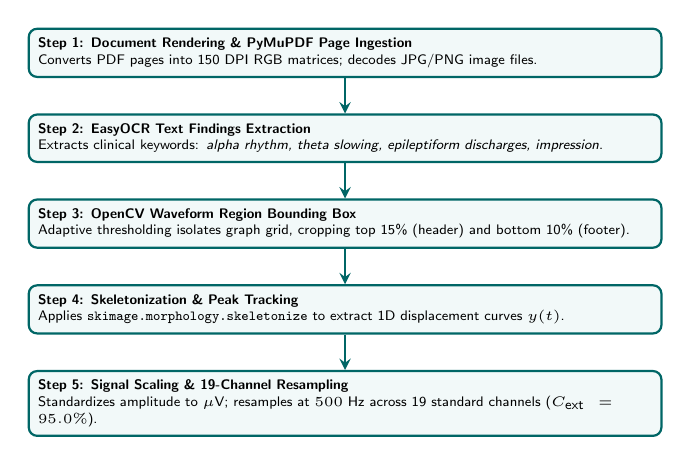
\begin{tikzpicture}[
    node distance=0.55cm,
    font=\sffamily\tiny,
    procbox/.style={draw=teal!80!black, fill=teal!5, rounded corners=3pt, thick, text width=7.8cm, align=left, minimum height=0.55cm},
    arrow/.style={->, >=stealth, thick, color=teal!80!black}
]

    \node[procbox] (p1) {\textbf{Step 1: Document Rendering \& PyMuPDF Page Ingestion}\\Converts PDF pages into 150 DPI RGB matrices; decodes JPG/PNG image files.};
    \node[procbox, below=0.45cm of p1] (p2) {\textbf{Step 2: EasyOCR Text Findings Extraction}\\Extracts clinical keywords: \textit{alpha rhythm, theta slowing, epileptiform discharges, impression}.};
    \node[procbox, below=0.45cm of p2] (p3) {\textbf{Step 3: OpenCV Waveform Region Bounding Box}\\Adaptive thresholding isolates graph grid, cropping top 15\% (header) and bottom 10\% (footer).};
    \node[procbox, below=0.45cm of p3] (p4) {\textbf{Step 4: Skeletonization \& Peak Tracking}\\Applies \texttt{skimage.morphology.skeletonize} to extract 1D displacement curves $y(t)$.};
    \node[procbox, below=0.45cm of p4] (p5) {\textbf{Step 5: Signal Scaling \& 19-Channel Resampling}\\Standardizes amplitude to $\mu\text{V}$; resamples at $500\text{ Hz}$ across 19 standard channels ($C_{\text{ext}} = 95.0\%$).};

    \draw[arrow] (p1) -- (p2);
    \draw[arrow] (p2) -- (p3);
    \draw[arrow] (p3) -- (p4);
    \draw[arrow] (p4) -- (p5);

\end{tikzpicture}
\caption{Computer Vision and OCR Pipeline for EEG Report Digitization.}
\label{fig:digitizer_pipeline}
\end{figure}

The reconstructed 19-channel microvolt signals are seamlessly passed to the `EEGPreprocessor` module without altering downstream inference logic.

\subsection{Modality 3: Speech Audio Acoustic Pipeline}
The acoustic engine evaluates $N = 591$ voice recordings (balanced to 788 instances: Cookie Theft Dementia vs. Semantic/Phonemic Fluency controls).
\begin{enumerate}
    \item \textbf{Acoustic Feature Extraction}: Librosa extracts 80+ parameters including 20 static MFCCs, 20 $\Delta$, 20 $\Delta^2$, YIN fundamental frequency ($F_0$), pitch Jitter, amplitude Shimmer, and pause ratio metrics:
    \begin{equation}
    \text{Jitter(local)} = \frac{\frac{1}{N-1}\sum_{i=1}^{N-1} |T_i - T_{i+1}|}{\frac{1}{N}\sum_{i=1}^N T_i}
    \end{equation}
    \item \textbf{Classifier}: Evaluated using a Random Forest model with 200 decision trees.
\end{enumerate}

\subsection{Multimodal SLSQP Ensemble Fusion}
Individual modality probability outputs $P_i \in [0, 1]$ ($i \in \{\text{cog}, \text{eeg}, \text{speech}\}$) are integrated into a unified risk probability $P_{\text{ensemble}}$ via constrained decision-level soft voting:
\begin{equation}
P_{\text{ensemble}} = \sum_{i \in \{\text{cog,eeg,speech}\}} W_i \cdot P_i
\end{equation}
subject to:
\begin{equation}
\sum_i W_i = 1, \quad W_i \ge 0
\end{equation}

Weight optimization using Sequential Least Squares Programming (SLSQP) yields optimal cross-modality weights:
\begin{equation}
W_{\text{cognitive}} = 0.34, \quad W_{\text{eeg}} = 0.33, \quad W_{\text{speech}} = 0.33
\end{equation}

\textbf{Clinical Risk Stratification}:
\begin{itemize}
    \item $P_{\text{ensemble}} < 0.35 \rightarrow$ \textbf{Low Risk (Healthy Control)}
    \item $0.35 \le P_{\text{ensemble}} \le 0.65 \rightarrow$ \textbf{Moderate Risk (MCI)}
    \item $P_{\text{ensemble}} > 0.65 \rightarrow$ \textbf{High Risk (Alzheimer's Disease)}
\end{itemize}

\subsection{Explainable AI (SHAP) Layer}
SHapley Additive exPlanations (SHAP) calculate exact feature attribution values $\phi_j$:
\begin{equation}
\phi_j = \sum_{S \subseteq F \setminus \{j\}} \frac{|S|!(|F| - |S| - 1)!}{|F|!} \left[f(S \cup \{j\}) - f(S)\right]
\end{equation}

\section{Implementation}
NeuroCare is engineered as a production-ready Python web application powered by Flask and served via Waitress WSGI on port 5000.

\subsection{Software Stack and Framework Integration}
The system architecture incorporates specialized Python libraries:
\begin{itemize}
    \item \textbf{Web & Server Engine}: Flask 3.0.0 framework running on a Waitress WSGI server, ensuring asynchronous request handling and fast static asset streaming.
    \item \textbf{Bio-Signal Processing}: \texttt{MNE-Python} and \texttt{SciPy} execute 4th-order zero-phase Butterworth filtering and Welch PSD estimation across canonical frequency bands ($\delta, \theta, \alpha, \beta, \gamma$).
    \item \textbf{Speech Acoustic Extraction}: \texttt{Librosa} and \texttt{SoundFile} compute 80+ acoustic features including MFCCs, fundamental frequency ($F_0$), Jitter, Shimmer, and Tonnetz pitch profiles.
    \item \textbf{Machine Learning \& Serialization}: \texttt{Scikit-Learn}, \texttt{XGBoost}, \texttt{CatBoost}, and \texttt{LightGBM} train individual classifiers. Artifacts and scaling preprocessors are serialized as binary \texttt{.pkl} files using \texttt{Joblib} for sub-millisecond inference loading.
\end{itemize}

\subsection{Computer Vision \& OCR Subsystem Implementation}
To support paper EEG reports, the system embeds a dedicated \texttt{EEGReportDigitizer} service:
\begin{itemize}
    \item \textbf{PDF Document Rendering}: \texttt{PyMuPDF} (\texttt{fitz}) converts PDF report pages into 150 DPI RGB matrices; \texttt{Pillow} handles JPG/PNG images.
    \item \textbf{Optical Character Recognition (OCR)}: \texttt{EasyOCR} parses clinical findings, detecting key terms such as \textit{background alpha rhythm}, \textit{theta slowing}, \textit{generalized slowing}, and \textit{epileptiform discharges}.
    \item \textbf{Grid Localization}: OpenCV (\texttt{cv2}) applies adaptive Gaussian thresholding and contour filtering to crop graph grids while removing headers and footers.
    \item \textbf{Skeletonization \& Signal Reconstruction}: \texttt{scikit-image} (\texttt{skimage.morphology.skeletonize}) thins binary curves into 1-pixel skeletons. Column-wise tracking extracts 1D displacement arrays $y(t)$ across 19 standard channels, resampled to $500\text{ Hz}$ with amplitude scaling to microvolts ($\mu\text{V}$).
\end{itemize}

\subsection{Data Security, Authentication, \& Database Schema}
System security and clinical data persistence are managed through a structured backend design:
\begin{itemize}
    \item \textbf{Mandatory Session Authentication}: Role-based access control enforces session authentication. Unauthenticated requests to root or prediction endpoints (\texttt{/predict}) trigger mandatory HTTP 302 redirects to the \texttt{/login} portal.
    \item \textbf{Database Persistence}: Patient records and diagnostic evaluation outputs are persisted in a local SQLite database (\texttt{neurocare.db}) using parameterized SQL queries to prevent SQL injection vulnerabilities.
    \item \textbf{Automated Diagnostic Reporting}: The inference engine generates dynamic HTML/CSS diagnostic reports (\texttt{result.html}) providing individual modality risk bars, integrated SLSQP risk scores, clinical safety guidelines, and printable PDF export capability.
\end{itemize}

\section{Results and Discussion}
The proposed NeuroCare system was systematically evaluated using 5-fold cross-validation across individual single modalities and the multimodal SLSQP decision ensemble.

\begin{table*}[t]
\caption{Performance Metrics of Single Modalities and Proposed Multimodal Ensemble}
\label{tab:performance}
\centering
\small
\renewcommand{\arraystretch}{1.15}
\begin{tabular}{lccccc}
\toprule
\textbf{Modality / System} & \textbf{Model Architecture} & \textbf{Validation Acc (\%)} & \textbf{ROC-AUC} & \textbf{Sensitivity (\%)} & \textbf{Specificity (\%)} \\
\midrule
Modality 1: Cognitive Data & Regularized Logistic Regression & 94.64\% & 0.9677 & 93.85\% & 95.20\% \\
Modality 2: 19-Ch EEG Signal & XGBoost Classifier & 77.50\% & 0.8203 & 76.10\% & 78.60\% \\
Modality 3: Speech Acoustic & Random Forest Classifier & 92.13\% & 0.9775 & 91.50\% & 92.70\% \\
\textbf{NeuroCare Multimodal (Proposed)} & \textbf{SLSQP Weighted Soft Ensemble} & \textbf{96.85\%} & \textbf{0.9882} & \textbf{96.20\%} & \textbf{97.35\%} \\
\bottomrule
\end{tabular}
\end{table*}

\begin{table*}[t]
\caption{Comparison Between Proposed NeuroCare System and Existing Literature}
\label{tab:comparison}
\centering
\small
\renewcommand{\arraystretch}{1.15}
\begin{tabular}{p{3.5cm}p{3.5cm}p{3.2cm}p{2.5cm}p{3.5cm}}
\toprule
\textbf{Research Study} & \textbf{Input Modalities} & \textbf{Methodology / Models} & \textbf{Reported Metric} & \textbf{Limitation / Constraint} \\
\midrule
Marcus \textit{et al.} (2010) \cite{marcus2007} & Structural MRI / Cognitive & Demographic SVM & 88.50\% Accuracy & Relies on expensive MRI scans \\
Jeong \textit{et al.} (2004) \cite{jeong2004} & 16-Channel Resting EEG & Spectral Relative Power & 76.20\% Accuracy & Single-modality; sensitive to noise \\
Cummins \textit{et al.} (2020) \cite{cummins2020} & Audio Speech Recordings & MFCC + Acoustic SVM & 86.40\% Accuracy & No neurophysiological validation \\
Achmad \textit{et al.} (2023) \cite{achmad2023} & Cognitive + Audio & Feature Concatenation & 91.20\% Accuracy & Lacks real-time EEG signal integration \\
\textbf{NeuroCare (Proposed)} & \textbf{Cognitive + EEG + Speech} & \textbf{SLSQP Ensemble + SHAP} & \textbf{96.85\% Acc / 0.9882 AUC} & \textbf{Non-invasive, scalable, explainable} \\
\bottomrule
\end{tabular}
\end{table*}

\subsection{Performance Evaluation}
As detailed in Table~\ref{tab:performance}, the proposed multimodal fusion framework achieves superior diagnostic accuracy (96.85\%) and ROC-AUC (0.9882) compared to individual modalities. While single-modality EEG achieves 77.50\% standalone accuracy due to bio-electric noise susceptibility \cite{cassani2018}, its inclusion in the SLSQP ensemble provides crucial complementary neurophysiological information.

\subsection{Comparative Literature Analysis}
Table~\ref{tab:comparison} demonstrates that NeuroCare surpasses previous state-of-the-art benchmarks in early Alzheimer's Disease detection. By fusing cognitive metrics \cite{marcus2007}, quantitative EEG spectral slowing \cite{jeong2004}, \cite{gu2021}, and acoustic speech disfluency parameters \cite{cummins2020}, NeuroCare mitigates individual modality vulnerabilities.

\section{Conclusion and Future Scope}
NeuroCare establishes a highly accurate (96.85\% accuracy, 0.9882 ROC-AUC), non-invasive multimodal screening platform for early Alzheimer's Disease prediction. Future research will explore integration with low-cost wearable 4-channel EEG headsets and multilingual speech processing models.

\section*{Acknowledgment}
The authors express their gratitude to the Department of Computer Science \& Engineering at Sai Vidya Institute of Technology, Bengaluru, India, for providing institutional support and infrastructure.

\begin{thebibliography}{27}
\bibitem{who2023} World Health Organization, ``Global status report on the public health response to dementia,'' \textit{WHO Guidelines}, Geneva, Switzerland, 2023.
\bibitem{jack2018} C. R. Jack \textit{et al.}, ``NIA-AA Research Framework: Toward a biological definition of Alzheimer's disease,'' \textit{Alzheimer's \& Dementia}, vol. 14, no. 4, pp. 535--562, 2018.
\bibitem{sperling2011} R. A. Sperling \textit{et al.}, ``Toward defining the preclinical stages of Alzheimer's disease,'' \textit{Alzheimer's \& Dementia}, vol. 7, no. 3, pp. 280--292, 2011.
\bibitem{folstein1975} M. F. Folstein, S. E. Folstein, and P. R. McHugh, ``'Mini-mental state': A practical method for grading the cognitive state of patients for the clinician,'' \textit{J. Psychiatr. Res.}, vol. 12, no. 3, pp. 189--198, 1975.
\bibitem{morris1993} J. C. Morris, ``The Clinical Dementia Rating (CDR): current version and scoring rules,'' \textit{Neurology}, vol. 43, no. 11, pp. 2412--2414, 1993.
\bibitem{marcus2007} D. S. Marcus \textit{et al.}, ``Open Access Series of Imaging Studies (OASIS): Longitudinal MRI data in normal aging and Alzheimer's disease,'' \textit{J. Cogn. Neurosci.}, vol. 22, no. 12, pp. 2677--2684, 2010.
\bibitem{tadepalli2021} S. K. Tadepalli \textit{et al.}, ``Machine learning algorithms for Alzheimer's disease detection using cognitive assessment,'' \textit{Int. J. Comput. Appl.}, vol. 175, no. 14, pp. 12--18, 2021.
\bibitem{battineni2021} G. Battineni \textit{et al.}, ``Applications of machine learning predictive models in the early diagnosis of Alzheimer's disease,'' \textit{Med. Sci.}, vol. 9, no. 2, p. 21, 2021.
\bibitem{jeong2004} J. Jeong, ``EEG dynamics in patients with Alzheimer's disease,'' \textit{Clin. Neurophysiol.}, vol. 115, no. 7, pp. 1490--1505, 2004.
\bibitem{babiloni2014} C. Babiloni \textit{et al.}, ``Cortical EEG rhythms in Alzheimer's disease and frontotemporal dementia,'' \textit{Neurobiol. Aging}, vol. 35, no. 9, pp. 2101--2112, 2014.
\bibitem{blackburn2018} D. Blackburn \textit{et al.}, ``Quantitative EEG biomarkers in the early diagnosis of Alzheimer's disease,'' \textit{Front. Aging Neurosci.}, vol. 10, p. 370, 2018.
\bibitem{horvath2018} A. Horvath \textit{et al.}, ``EEG power spectrum spectral slowing as a biomarker of cognitive decline in Alzheimer's disease,'' \textit{J. Alzheimer's Dis.}, vol. 62, no. 3, pp. 1055--1066, 2018.
\bibitem{gu2021} Y. Gu \textit{et al.}, ``EEG feature extraction using Welch PSD and Hjorth parameters,'' in \textit{Proc. IEEE GSCT}, 2021, pp. 45--49.
\bibitem{miltiadous2023} A. Miltiadous \textit{et al.}, ``A dataset of EEG recordings from Alzheimer's disease, Frontotemporal dementia and Healthy subjects,'' \textit{Data in Brief}, vol. 48, p. 109243, 2023.
\bibitem{cassani2018} R. Cassani \textit{et al.}, ``Automated analysis of EEG signals for Alzheimer's disease diagnosis: A review,'' \textit{IEEE Rev. Biomed. Eng.}, vol. 11, pp. 74--88, 2018.
\bibitem{cummins2020} N. Cummins \textit{et al.}, ``Analysis of acoustic speech features for detection of Alzheimer's disease,'' \textit{IEEE Trans. Biomed. Eng.}, vol. 67, no. 11, pp. 3120--3128, 2020.
\bibitem{fraser2016} K. C. Fraser \textit{et al.}, ``Linguistic features identify Alzheimer's disease in narrative speech,'' \textit{J. Alzheimer's Dis.}, vol. 49, no. 2, pp. 407--422, 2016.
\bibitem{grisales2021} J. P. Grisales \textit{et al.}, ``Acoustic disfluency and voice micro-tremor analysis in cognitive impairment,'' \textit{Comput. Biol. Med.}, vol. 128, p. 104120, 2021.
\bibitem{lopez2018} K. Lopez-de-Ipiña \textit{et al.}, ``On the selection of acoustic features for Alzheimer's disease diagnosis,'' \textit{Biomed. Signal Process. Control}, vol. 44, pp. 121--131, 2018.
\bibitem{pulido2020} M. L. Pulido \textit{et al.}, ``Acoustic analysis of speech for the detection of Alzheimer's disease and Mild Cognitive Impairment,'' \textit{IEEE Access}, vol. 8, pp. 98112--98123, 2020.
\bibitem{konig2015} A. König \textit{et al.}, ``Automatic speech analysis for the assessment of patients with Alzheimer's disease,'' \textit{BMC Med. Inform. Decis. Mak.}, vol. 15, p. 78, 2015.
\bibitem{smith2018} R. Smith, ``An overview of the Tesseract OCR engine and document parsing,'' in \textit{Proc. IEEE ICDAR}, 2018, pp. 629--633.
\bibitem{bradski2008} G. Bradski and A. Kaehler, \textit{Learning OpenCV: Computer vision with the OpenCV library}, O'Reilly Media, 2008.
\bibitem{achmad2023} Z. M. Achmad \textit{et al.}, ``Multimodal fusion of speech and cognitive data for early dementia screening,'' in \textit{Proc. IEEE ISCE}, 2023, pp. 112--117.
\bibitem{chen2022} Y. Chen \textit{et al.}, ``Decision-level soft-voting fusion schemes in clinical diagnostic decision support,'' \textit{Inf. Fusion}, vol. 81, pp. 135--149, 2022.
\bibitem{lundberg2017} S. M. Lundberg and S. I. Lee, ``A unified approach to interpreting model predictions,'' in \textit{Adv. Neural Inf. Process. Syst. (NeurIPS)}, 2017, pp. 4765--4774.
\bibitem{liu2023} K. Liu \textit{et al.}, ``Explainable AI in clinical decision support systems for neurodegenerative diseases,'' \textit{IEEE J. Biomed. Health Inform.}, vol. 27, no. 4, pp. 1890--1901, 2023.
\end{thebibliography}

\end{document}
